% Created by tikzDevice version 0.12.3.1 on 2021-12-04 19:34:20
% !TEX encoding = UTF-8 Unicode
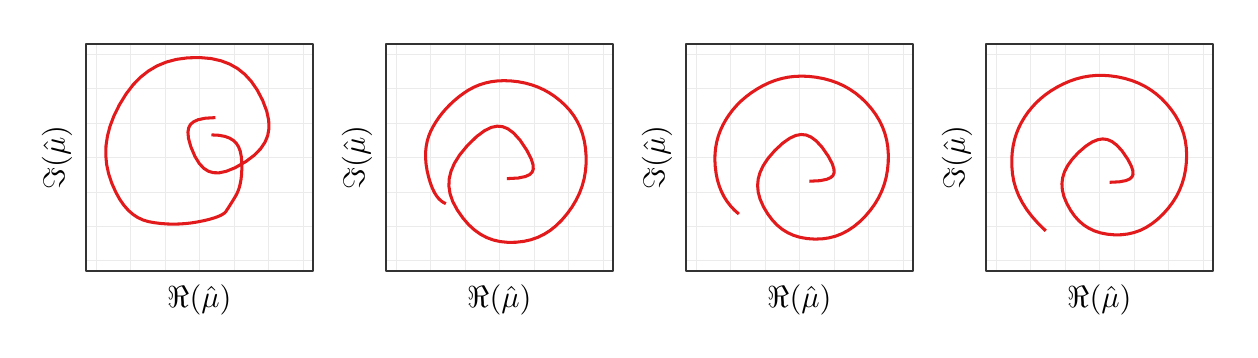
\begin{tikzpicture}[x=1pt,y=1pt]
\definecolor{fillColor}{RGB}{255,255,255}
\begin{scope}
\definecolor{drawColor}{RGB}{255,255,255}
\definecolor{fillColor}{RGB}{255,255,255}

\path[draw=drawColor,line width= 0.6pt,line join=round,line cap=round,fill=fillColor] ( -0.00,  0.00) rectangle (108.41,108.41);
\end{scope}
\begin{scope}
\definecolor{fillColor}{RGB}{255,255,255}

\path[fill=fillColor] ( 20.71, 20.71) rectangle (102.91,102.91);
\definecolor{drawColor}{gray}{0.92}

\path[draw=drawColor,line width= 0.3pt,line join=round] ( 20.71, 24.45) --
	(102.91, 24.45);

\path[draw=drawColor,line width= 0.3pt,line join=round] ( 20.71, 49.36) --
	(102.91, 49.36);

\path[draw=drawColor,line width= 0.3pt,line join=round] ( 20.71, 74.26) --
	(102.91, 74.26);

\path[draw=drawColor,line width= 0.3pt,line join=round] ( 20.71, 99.17) --
	(102.91, 99.17);

\path[draw=drawColor,line width= 0.3pt,line join=round] ( 24.45, 20.71) --
	( 24.45,102.91);

\path[draw=drawColor,line width= 0.3pt,line join=round] ( 49.36, 20.71) --
	( 49.36,102.91);

\path[draw=drawColor,line width= 0.3pt,line join=round] ( 74.26, 20.71) --
	( 74.26,102.91);

\path[draw=drawColor,line width= 0.3pt,line join=round] ( 99.17, 20.71) --
	( 99.17,102.91);

\path[draw=drawColor,line width= 0.6pt,line join=round] ( 20.71, 36.90) --
	(102.91, 36.90);

\path[draw=drawColor,line width= 0.6pt,line join=round] ( 20.71, 61.81) --
	(102.91, 61.81);

\path[draw=drawColor,line width= 0.6pt,line join=round] ( 20.71, 86.72) --
	(102.91, 86.72);

\path[draw=drawColor,line width= 0.6pt,line join=round] ( 36.90, 20.71) --
	( 36.90,102.91);

\path[draw=drawColor,line width= 0.6pt,line join=round] ( 61.81, 20.71) --
	( 61.81,102.91);

\path[draw=drawColor,line width= 0.6pt,line join=round] ( 86.72, 20.71) --
	( 86.72,102.91);
\definecolor{drawColor}{RGB}{227,26,28}

\path[draw=drawColor,line width= 1.1pt,line join=round] ( 67.55, 76.21) --
	( 63.85, 75.99) --
	( 61.29, 75.45) --
	( 59.60, 74.68) --
	( 58.52, 73.72) --
	( 57.87, 72.52) --
	( 57.61, 70.93) --
	( 57.81, 68.73) --
	( 58.65, 65.70) --
	( 60.15, 62.17) --
	( 61.73, 59.60) --
	( 63.33, 57.90) --
	( 64.98, 56.84) --
	( 66.79, 56.30) --
	( 68.89, 56.26) --
	( 71.44, 56.80) --
	( 74.61, 58.08) --
	( 78.43, 60.26) --
	( 81.61, 62.64) --
	( 83.90, 64.99) --
	( 85.47, 67.34) --
	( 86.45, 69.76) --
	( 86.89, 72.36) --
	( 86.79, 75.26) --
	( 86.07, 78.58) --
	( 84.60, 82.45) --
	( 82.61, 86.25) --
	( 80.45, 89.37) --
	( 78.11, 91.90) --
	( 75.55, 93.94) --
	( 72.73, 95.54) --
	( 69.58, 96.74) --
	( 66.01, 97.55) --
	( 61.92, 97.91) --
	( 57.47, 97.81) --
	( 53.44, 97.25) --
	( 49.80, 96.28) --
	( 46.48, 94.91) --
	( 43.41, 93.11) --
	( 40.54, 90.87) --
	( 37.83, 88.11) --
	( 35.26, 84.76) --
	( 32.83, 80.80) --
	( 30.88, 76.85) --
	( 29.46, 73.11) --
	( 28.52, 69.53) --
	( 28.01, 66.07) --
	( 27.92, 62.69) --
	( 28.22, 59.33) --
	( 28.94, 55.95) --
	( 30.10, 52.50) --
	( 31.52, 49.30) --
	( 33.00, 46.63) --
	( 34.54, 44.43) --
	( 36.14, 42.64) --
	( 37.80, 41.20) --
	( 39.56, 40.06) --
	( 41.43, 39.20) --
	( 43.46, 38.60) --
	( 45.64, 38.22) --
	( 47.83, 37.95) --
	( 50.02, 37.78) --
	( 52.21, 37.72) --
	( 54.41, 37.77) --
	( 56.63, 37.91) --
	( 58.86, 38.16) --
	( 61.12, 38.52) --
	( 63.39, 38.98) --
	( 65.36, 39.46) --
	( 66.97, 39.93) --
	( 68.27, 40.38) --
	( 69.29, 40.81) --
	( 70.07, 41.22) --
	( 70.65, 41.60) --
	( 71.06, 41.96) --
	( 71.34, 42.29) --
	( 71.57, 42.65) --
	( 71.85, 43.07) --
	( 72.17, 43.56) --
	( 72.53, 44.13) --
	( 72.94, 44.78) --
	( 73.41, 45.53) --
	( 73.93, 46.36) --
	( 74.50, 47.30) --
	( 75.11, 48.34) --
	( 75.65, 49.49) --
	( 76.11, 50.77) --
	( 76.49, 52.20) --
	( 76.78, 53.78) --
	( 76.98, 55.55) --
	( 77.08, 57.51) --
	( 77.06, 59.69) --
	( 76.90, 62.05) --
	( 76.51, 64.07) --
	( 75.90, 65.67) --
	( 75.08, 66.94) --
	( 74.03, 67.96) --
	( 72.71, 68.78) --
	( 71.01, 69.41) --
	( 68.85, 69.82) --
	( 66.11, 69.97);
\definecolor{drawColor}{gray}{0.20}

\path[draw=drawColor,line width= 0.6pt,line join=round,line cap=round] ( 20.71, 20.71) rectangle (102.91,102.91);
\end{scope}
\begin{scope}
\definecolor{drawColor}{RGB}{0,0,0}

\node[text=drawColor,anchor=base,inner sep=0pt, outer sep=0pt, scale=  1.10] at ( 61.81,  7.64) {$\Re(\hat\mu)$};
\end{scope}
\begin{scope}
\definecolor{drawColor}{RGB}{0,0,0}

\node[text=drawColor,rotate= 90.00,anchor=base,inner sep=0pt, outer sep=0pt, scale=  1.10] at ( 13.08, 61.81) {$\Im(\hat\mu)$};
\end{scope}
\begin{scope}
\definecolor{drawColor}{RGB}{255,255,255}
\definecolor{fillColor}{RGB}{255,255,255}

\path[draw=drawColor,line width= 0.6pt,line join=round,line cap=round,fill=fillColor] (108.41,  0.00) rectangle (216.81,108.41);
\end{scope}
\begin{scope}
\definecolor{fillColor}{RGB}{255,255,255}

\path[fill=fillColor] (129.12, 20.71) rectangle (211.31,102.91);
\definecolor{drawColor}{gray}{0.92}

\path[draw=drawColor,line width= 0.3pt,line join=round] (129.12, 24.45) --
	(211.31, 24.45);

\path[draw=drawColor,line width= 0.3pt,line join=round] (129.12, 49.36) --
	(211.31, 49.36);

\path[draw=drawColor,line width= 0.3pt,line join=round] (129.12, 74.26) --
	(211.31, 74.26);

\path[draw=drawColor,line width= 0.3pt,line join=round] (129.12, 99.17) --
	(211.31, 99.17);

\path[draw=drawColor,line width= 0.3pt,line join=round] (132.86, 20.71) --
	(132.86,102.91);

\path[draw=drawColor,line width= 0.3pt,line join=round] (157.76, 20.71) --
	(157.76,102.91);

\path[draw=drawColor,line width= 0.3pt,line join=round] (182.67, 20.71) --
	(182.67,102.91);

\path[draw=drawColor,line width= 0.3pt,line join=round] (207.57, 20.71) --
	(207.57,102.91);

\path[draw=drawColor,line width= 0.6pt,line join=round] (129.12, 36.90) --
	(211.31, 36.90);

\path[draw=drawColor,line width= 0.6pt,line join=round] (129.12, 61.81) --
	(211.31, 61.81);

\path[draw=drawColor,line width= 0.6pt,line join=round] (129.12, 86.72) --
	(211.31, 86.72);

\path[draw=drawColor,line width= 0.6pt,line join=round] (145.31, 20.71) --
	(145.31,102.91);

\path[draw=drawColor,line width= 0.6pt,line join=round] (170.21, 20.71) --
	(170.21,102.91);

\path[draw=drawColor,line width= 0.6pt,line join=round] (195.12, 20.71) --
	(195.12,102.91);
\definecolor{drawColor}{RGB}{227,26,28}

\path[draw=drawColor,line width= 1.1pt,line join=round] (172.84, 54.16) --
	(176.89, 54.37) --
	(179.52, 54.91) --
	(181.11, 55.64) --
	(181.98, 56.50) --
	(182.39, 57.58) --
	(182.34, 59.09) --
	(181.66, 61.28) --
	(180.06, 64.41) --
	(177.59, 68.10) --
	(175.29, 70.64) --
	(173.22, 72.17) --
	(171.29, 72.95) --
	(169.35, 73.12) --
	(167.25, 72.69) --
	(164.82, 71.51) --
	(161.93, 69.37) --
	(158.55, 66.07) --
	(155.79, 62.71) --
	(153.87, 59.63) --
	(152.65, 56.77) --
	(152.01, 54.07) --
	(151.91, 51.42) --
	(152.32, 48.73) --
	(153.29, 45.90) --
	(154.92, 42.86) --
	(156.94, 39.97) --
	(158.99, 37.58) --
	(161.10, 35.64) --
	(163.27, 34.09) --
	(165.53, 32.88) --
	(167.93, 31.99) --
	(170.49, 31.41) --
	(173.29, 31.13) --
	(176.24, 31.18) --
	(178.99, 31.50) --
	(181.55, 32.08) --
	(183.96, 32.92) --
	(186.24, 34.02) --
	(188.44, 35.40) --
	(190.56, 37.08) --
	(192.63, 39.10) --
	(194.64, 41.47) --
	(196.41, 43.93) --
	(197.88, 46.40) --
	(199.08, 48.89) --
	(200.04, 51.42) --
	(200.75, 54.01) --
	(201.23, 56.69) --
	(201.48, 59.47) --
	(201.48, 62.38) --
	(201.25, 65.24) --
	(200.81, 67.89) --
	(200.18, 70.34) --
	(199.35, 72.63) --
	(198.33, 74.77) --
	(197.10, 76.80) --
	(195.67, 78.72) --
	(194.00, 80.56) --
	(192.13, 82.29) --
	(190.19, 83.82) --
	(188.20, 85.15) --
	(186.14, 86.30) --
	(183.99, 87.27) --
	(181.75, 88.07) --
	(179.40, 88.71) --
	(176.92, 89.18) --
	(174.31, 89.47) --
	(171.79, 89.56) --
	(169.42, 89.46) --
	(167.18, 89.18) --
	(165.05, 88.71) --
	(163.00, 88.07) --
	(161.04, 87.25) --
	(159.12, 86.24) --
	(157.26, 85.03) --
	(155.47, 83.70) --
	(153.82, 82.32) --
	(152.29, 80.90) --
	(150.87, 79.43) --
	(149.56, 77.91) --
	(148.35, 76.34) --
	(147.24, 74.71) --
	(146.23, 73.02) --
	(145.32, 71.27) --
	(144.60, 69.48) --
	(144.06, 67.65) --
	(143.69, 65.74) --
	(143.49, 63.76) --
	(143.48, 61.67) --
	(143.65, 59.45) --
	(144.02, 57.10) --
	(144.60, 54.62) --
	(145.27, 52.42) --
	(145.97, 50.59) --
	(146.71, 49.09) --
	(147.47, 47.88) --
	(148.26, 46.91) --
	(149.06, 46.14) --
	(149.91, 45.56) --
	(150.80, 45.12);
\definecolor{drawColor}{gray}{0.20}

\path[draw=drawColor,line width= 0.6pt,line join=round,line cap=round] (129.12, 20.71) rectangle (211.31,102.91);
\end{scope}
\begin{scope}
\definecolor{drawColor}{RGB}{0,0,0}

\node[text=drawColor,anchor=base,inner sep=0pt, outer sep=0pt, scale=  1.10] at (170.21,  7.64) {$\Re(\hat\mu)$};
\end{scope}
\begin{scope}
\definecolor{drawColor}{RGB}{0,0,0}

\node[text=drawColor,rotate= 90.00,anchor=base,inner sep=0pt, outer sep=0pt, scale=  1.10] at (121.48, 61.81) {$\Im(\hat\mu)$};
\end{scope}
\begin{scope}
\definecolor{drawColor}{RGB}{255,255,255}
\definecolor{fillColor}{RGB}{255,255,255}

\path[draw=drawColor,line width= 0.6pt,line join=round,line cap=round,fill=fillColor] (216.81,  0.00) rectangle (325.22,108.41);
\end{scope}
\begin{scope}
\definecolor{fillColor}{RGB}{255,255,255}

\path[fill=fillColor] (237.52, 20.71) rectangle (319.72,102.91);
\definecolor{drawColor}{gray}{0.92}

\path[draw=drawColor,line width= 0.3pt,line join=round] (237.52, 24.45) --
	(319.71, 24.45);

\path[draw=drawColor,line width= 0.3pt,line join=round] (237.52, 49.36) --
	(319.71, 49.36);

\path[draw=drawColor,line width= 0.3pt,line join=round] (237.52, 74.26) --
	(319.71, 74.26);

\path[draw=drawColor,line width= 0.3pt,line join=round] (237.52, 99.17) --
	(319.71, 99.17);

\path[draw=drawColor,line width= 0.3pt,line join=round] (241.26, 20.71) --
	(241.26,102.91);

\path[draw=drawColor,line width= 0.3pt,line join=round] (266.17, 20.71) --
	(266.17,102.91);

\path[draw=drawColor,line width= 0.3pt,line join=round] (291.07, 20.71) --
	(291.07,102.91);

\path[draw=drawColor,line width= 0.3pt,line join=round] (315.98, 20.71) --
	(315.98,102.91);

\path[draw=drawColor,line width= 0.6pt,line join=round] (237.52, 36.90) --
	(319.71, 36.90);

\path[draw=drawColor,line width= 0.6pt,line join=round] (237.52, 61.81) --
	(319.71, 61.81);

\path[draw=drawColor,line width= 0.6pt,line join=round] (237.52, 86.72) --
	(319.71, 86.72);

\path[draw=drawColor,line width= 0.6pt,line join=round] (253.71, 20.71) --
	(253.71,102.91);

\path[draw=drawColor,line width= 0.6pt,line join=round] (278.62, 20.71) --
	(278.62,102.91);

\path[draw=drawColor,line width= 0.6pt,line join=round] (303.53, 20.71) --
	(303.53,102.91);
\definecolor{drawColor}{RGB}{227,26,28}

\path[draw=drawColor,line width= 1.1pt,line join=round] (282.16, 53.22) --
	(285.97, 53.42) --
	(288.43, 53.91) --
	(289.91, 54.56) --
	(290.72, 55.33) --
	(291.09, 56.28) --
	(291.05, 57.59) --
	(290.44, 59.52) --
	(288.99, 62.27) --
	(286.73, 65.53) --
	(284.63, 67.80) --
	(282.73, 69.20) --
	(280.96, 69.93) --
	(279.20, 70.11) --
	(277.31, 69.78) --
	(275.15, 68.81) --
	(272.61, 67.04) --
	(269.66, 64.30) --
	(267.23, 61.47) --
	(265.49, 58.85) --
	(264.33, 56.37) --
	(263.67, 54.00) --
	(263.46, 51.65) --
	(263.68, 49.25) --
	(264.37, 46.72) --
	(265.58, 43.99) --
	(267.14, 41.38) --
	(268.79, 39.18) --
	(270.52, 37.35) --
	(272.37, 35.84) --
	(274.34, 34.62) --
	(276.47, 33.66) --
	(278.81, 32.95) --
	(281.40, 32.49) --
	(284.16, 32.31) --
	(286.77, 32.40) --
	(289.22, 32.75) --
	(291.56, 33.35) --
	(293.80, 34.21) --
	(295.98, 35.34) --
	(298.12, 36.75) --
	(300.24, 38.49) --
	(302.34, 40.56) --
	(304.21, 42.75) --
	(305.81, 44.97) --
	(307.17, 47.25) --
	(308.30, 49.61) --
	(309.21, 52.05) --
	(309.91, 54.60) --
	(310.39, 57.28) --
	(310.66, 60.11) --
	(310.69, 62.94) --
	(310.50, 65.61) --
	(310.08, 68.13) --
	(309.44, 70.54) --
	(308.58, 72.86) --
	(307.50, 75.10) --
	(306.17, 77.29) --
	(304.58, 79.45) --
	(302.76, 81.53) --
	(300.86, 83.38) --
	(298.88, 85.01) --
	(296.81, 86.43) --
	(294.64, 87.67) --
	(292.35, 88.72) --
	(289.92, 89.59) --
	(287.33, 90.29) --
	(284.58, 90.80) --
	(281.89, 91.11) --
	(279.32, 91.20) --
	(276.83, 91.10) --
	(274.43, 90.81) --
	(272.09, 90.32) --
	(269.79, 89.65) --
	(267.52, 88.77) --
	(265.27, 87.69) --
	(263.11, 86.45) --
	(261.11, 85.14) --
	(259.27, 83.75) --
	(257.57, 82.29) --
	(256.00, 80.73) --
	(254.55, 79.08) --
	(253.22, 77.33) --
	(252.00, 75.47) --
	(250.91, 73.52) --
	(250.00, 71.55) --
	(249.26, 69.54) --
	(248.70, 67.49) --
	(248.31, 65.38) --
	(248.08, 63.20) --
	(248.02, 60.93) --
	(248.15, 58.56) --
	(248.46, 56.08) --
	(248.93, 53.74) --
	(249.57, 51.58) --
	(250.35, 49.58) --
	(251.28, 47.72) --
	(252.37, 45.99) --
	(253.62, 44.36) --
	(255.05, 42.82) --
	(256.68, 41.36);
\definecolor{drawColor}{gray}{0.20}

\path[draw=drawColor,line width= 0.6pt,line join=round,line cap=round] (237.52, 20.71) rectangle (319.72,102.91);
\end{scope}
\begin{scope}
\definecolor{drawColor}{RGB}{0,0,0}

\node[text=drawColor,anchor=base,inner sep=0pt, outer sep=0pt, scale=  1.10] at (278.62,  7.64) {$\Re(\hat\mu)$};
\end{scope}
\begin{scope}
\definecolor{drawColor}{RGB}{0,0,0}

\node[text=drawColor,rotate= 90.00,anchor=base,inner sep=0pt, outer sep=0pt, scale=  1.10] at (229.89, 61.81) {$\Im(\hat\mu)$};
\end{scope}
\begin{scope}
\definecolor{drawColor}{RGB}{255,255,255}
\definecolor{fillColor}{RGB}{255,255,255}

\path[draw=drawColor,line width= 0.6pt,line join=round,line cap=round,fill=fillColor] (325.21,  0.00) rectangle (433.62,108.41);
\end{scope}
\begin{scope}
\definecolor{fillColor}{RGB}{255,255,255}

\path[fill=fillColor] (345.93, 20.71) rectangle (428.12,102.91);
\definecolor{drawColor}{gray}{0.92}

\path[draw=drawColor,line width= 0.3pt,line join=round] (345.93, 24.45) --
	(428.12, 24.45);

\path[draw=drawColor,line width= 0.3pt,line join=round] (345.93, 49.36) --
	(428.12, 49.36);

\path[draw=drawColor,line width= 0.3pt,line join=round] (345.93, 74.26) --
	(428.12, 74.26);

\path[draw=drawColor,line width= 0.3pt,line join=round] (345.93, 99.17) --
	(428.12, 99.17);

\path[draw=drawColor,line width= 0.3pt,line join=round] (349.67, 20.71) --
	(349.67,102.91);

\path[draw=drawColor,line width= 0.3pt,line join=round] (374.57, 20.71) --
	(374.57,102.91);

\path[draw=drawColor,line width= 0.3pt,line join=round] (399.48, 20.71) --
	(399.48,102.91);

\path[draw=drawColor,line width= 0.3pt,line join=round] (424.38, 20.71) --
	(424.38,102.91);

\path[draw=drawColor,line width= 0.6pt,line join=round] (345.93, 36.90) --
	(428.12, 36.90);

\path[draw=drawColor,line width= 0.6pt,line join=round] (345.93, 61.81) --
	(428.12, 61.81);

\path[draw=drawColor,line width= 0.6pt,line join=round] (345.93, 86.72) --
	(428.12, 86.72);

\path[draw=drawColor,line width= 0.6pt,line join=round] (362.12, 20.71) --
	(362.12,102.91);

\path[draw=drawColor,line width= 0.6pt,line join=round] (387.02, 20.71) --
	(387.02,102.91);

\path[draw=drawColor,line width= 0.6pt,line join=round] (411.93, 20.71) --
	(411.93,102.91);
\definecolor{drawColor}{RGB}{227,26,28}

\path[draw=drawColor,line width= 1.1pt,line join=round] (390.67, 52.83) --
	(394.25, 53.01) --
	(396.57, 53.46) --
	(397.97, 54.07) --
	(398.74, 54.79) --
	(399.10, 55.66) --
	(399.08, 56.88) --
	(398.53, 58.64) --
	(397.22, 61.16) --
	(395.17, 64.16) --
	(393.24, 66.26) --
	(391.48, 67.58) --
	(389.83, 68.29) --
	(388.19, 68.51) --
	(386.43, 68.25) --
	(384.42, 67.44) --
	(382.07, 65.92) --
	(379.34, 63.55) --
	(377.08, 61.09) --
	(375.44, 58.78) --
	(374.34, 56.59) --
	(373.68, 54.45) --
	(373.43, 52.31) --
	(373.57, 50.10) --
	(374.13, 47.75) --
	(375.18, 45.20) --
	(376.54, 42.73) --
	(378.01, 40.64) --
	(379.58, 38.90) --
	(381.26, 37.45) --
	(383.09, 36.26) --
	(385.09, 35.30) --
	(387.29, 34.58) --
	(389.76, 34.09) --
	(392.41, 33.85) --
	(394.91, 33.88) --
	(397.28, 34.17) --
	(399.53, 34.69) --
	(401.70, 35.47) --
	(403.81, 36.51) --
	(405.89, 37.83) --
	(407.96, 39.45) --
	(410.02, 41.41) --
	(411.86, 43.48) --
	(413.44, 45.59) --
	(414.80, 47.76) --
	(415.93, 50.01) --
	(416.85, 52.35) --
	(417.57, 54.80) --
	(418.09, 57.38) --
	(418.40, 60.12) --
	(418.49, 62.86) --
	(418.35, 65.46) --
	(417.99, 67.93) --
	(417.42, 70.30) --
	(416.64, 72.59) --
	(415.63, 74.82) --
	(414.38, 77.02) --
	(412.88, 79.18) --
	(411.15, 81.28) --
	(409.33, 83.16) --
	(407.43, 84.82) --
	(405.43, 86.28) --
	(403.33, 87.56) --
	(401.10, 88.66) --
	(398.73, 89.59) --
	(396.19, 90.35) --
	(393.48, 90.94) --
	(390.82, 91.31) --
	(388.24, 91.48) --
	(385.74, 91.45) --
	(383.30, 91.22) --
	(380.90, 90.80) --
	(378.53, 90.18) --
	(376.17, 89.36) --
	(373.81, 88.33) --
	(371.53, 87.14) --
	(369.43, 85.87) --
	(367.50, 84.51) --
	(365.71, 83.05) --
	(364.06, 81.51) --
	(362.54, 79.86) --
	(361.13, 78.11) --
	(359.84, 76.23) --
	(358.68, 74.25) --
	(357.69, 72.23) --
	(356.88, 70.15) --
	(356.24, 68.02) --
	(355.76, 65.80) --
	(355.45, 63.50) --
	(355.30, 61.09) --
	(355.34, 58.56) --
	(355.56, 55.90) --
	(356.02, 53.27) --
	(356.75, 50.70) --
	(357.74, 48.16) --
	(359.03, 45.63) --
	(360.62, 43.09) --
	(362.56, 40.53) --
	(364.87, 37.93) --
	(367.59, 35.28);
\definecolor{drawColor}{gray}{0.20}

\path[draw=drawColor,line width= 0.6pt,line join=round,line cap=round] (345.93, 20.71) rectangle (428.12,102.91);
\end{scope}
\begin{scope}
\definecolor{drawColor}{RGB}{0,0,0}

\node[text=drawColor,anchor=base,inner sep=0pt, outer sep=0pt, scale=  1.10] at (387.02,  7.64) {$\Re(\hat\mu)$};
\end{scope}
\begin{scope}
\definecolor{drawColor}{RGB}{0,0,0}

\node[text=drawColor,rotate= 90.00,anchor=base,inner sep=0pt, outer sep=0pt, scale=  1.10] at (338.29, 61.81) {$\Im(\hat\mu)$};
\end{scope}
\end{tikzpicture}
